\documentclass[12pt,letter]{article}
\usepackage[utf8]{inputenc}
\usepackage{amsmath}
\usepackage{amsfonts}
\usepackage{amssymb}
\usepackage{graphicx}

\usepackage{hyperref}
\hypersetup{colorlinks=true}

\usepackage[numbers,sort&compress]{natbib}
\usepackage{hypernat}

\bibliographystyle{plainurl}

\author{Ruisheng Fu\\21421190\\CCNT Lab.
\and
Guanyu Guo\\21421189\\LIST Lab.
\and
Chen Sui\\21421183}
\title{NoSQLs in Cloud Computing}
\date{\today}

\begin{document}
\maketitle
\tableofcontents

\begin{abstract}
A lot of changes in database management system has been made since the inception of cloud computing. Such critical and increasing needs within cloud computing as scalability, elasticity and  processing a huge amount of data can be fulfilled by the NoSQL databases as opposed to RDBMS\footnote{Relational Database Management System}. In this report we have dived into several primary NoSQL databases used in leading cloud vendors, summarizing and discussing detailed techniques as well as analysis with comparisons.
\end{abstract}

\section{Introduction}
Cloud computing has been a evolving computing terminology that is very much in the public eye. It is its responsibility to manage and group remote servers that allow data storage and online access to various services. 

In the field of computing, the various advancements and aspects are key evidences that explain the reason why higher priorities are given to scalability, resource utilization and power savings, with respect to data storage, rather than consistency. The traditional RDBMSs offer functionalities like clustering, synchronization (always consistent), load balancing and structured querying. However, what classical RDBMS could not do so well is to scale\footnote{Scaling, in a google sense, means that an application runs on small commodity PC hardware, but supports essentially unbounded load as more PC’s are added. } to heavy workloads compared to NoSQL databases. As non-relational databases have cropped up both inside and outside the cloud, there comes heated debate around SQL and NoSQL.\citep{Bain2009}

The two solutions, manual sharding and caching, applied to classical SQL databases are not adequate enough to cope up with the modern web applications, thus agility can't be achieved. On the contrary, NoSQL databases is designed to handle such sort of problems. In those applications where high availability, speed, fault tolerance or consistency are needed, NoSQL is the choice, in that it is designed to scale out, to provide elasticity and to be highly available. The misleading term \textit{NoSQL} should be seen as the definition\citep{Unknown2012} that is "Next Generation Databases mostly addressing some of the points: being non-relational, distributed, open-source and horizontally scalable", and is mostly translated with "Not only SQL".

In this report, we firstly examine several major NoSQL databases implemented and used in cloud vendors like Google, Amazon, and Yahoo, along with description about the main ideas of each design. Afterwards, analysis towards different NoSQL databases and we present benchmarking of top NoSQL as a visualizing comparison. Finally, a brief summarization is included in conclusion and further studies as well as challenges is discussed.

\section{Major Streams} \label{majorstream}
Currently there are approximately 150 NoSQL databases categorized by data models into a bunch of classes.\citep{Unknown2012} We review certain amount of prevailing NoSQL databases through several aspects, including data model, partitions, availability, and consistency. 

Bigtable\citep{Chang2006} designed by Google describes the well-known data model, which gives clients dynamic control over data layout and format and has successfully provided a flexible, high-performance solution for many Google products. 
The Amazon Dynamo\citep{DeCandia2007} presents a highly available key-value storage system that some of Amazon's core services use to provide an ``always-on'' experience.
Cassandra\citep{LakshamAvinash2010} concludes design model and implementation part and claims that it is designed to achieve high write throughput and without sacrificing read efficiency, which is a combination of Bigtable and Dynamo. 
\citep{Silberstein2008} describes the motivation of PNUTS and table storage and replication layers, and at the end presents performance analysis with experimental results.  
Paper \citep{Melnik2010} describes the architecture and implementation of Dremel, and explains how it complements Map/Reduce-based computing. We present a novel columnar storage representation for nested records and discuss experiments on few-thousand node instances of the system.
\citep{Suter2012} makes a brief introduction to MongoDB with an installation guide, and mainly focus on the performance benchmark.

\subsection{Data Model} \label{datamodel}
The major data models adopted we are going to investigate are \textit{Wide Column Store} (Column Families), \textit{Document Store}, and \textit{Key Value Store}, whereas the minor ones (Graph Databases, Object Databases, etc.) are beyond our scope of discussion in this report. 

\paragraph*{Column Family Store}
Columnar databases are logically similar to tabular databases. The difference is that the data are  column-wise stored and retrieved.

Bigtable\citep{Chang2006} is a kind of sparse, distributed, persistent sorted map introduced by Google. It is indexed by three elements: row key, column key, and timestamp like this:
\[ (row:string, column:string, time:int64) \rightarrow string \]

Each value in this map is an uninterpreted array of bytes. The row keys which is used to maintains data in lexicographic order are arbitrary strings. Column key consist of family and qualifier. Column keys are grouped into sets called column families, which form the basic unit of access control. Besides, Bigtable can contain multiple versions of each cell by indexed timestamp.

Similarly, Casandra comes under column family. Columns in Cassandra are grouped together very much similar to what happens in the Bigtable system. Cassandra\citep{LakshamAvinash2010} exposes two kinds of columns families, \textit{Simple} and \textit{Super} column families. Super column families can be visualized as a column family within a column family. Casandra also allows columns to be sorted either by time or by name, which is often exploited by different applications.

\paragraph*{Document Store}
A document-oriented database eschews the table-based relational database structure. MongoDB is the well-known member of the family. In general, it stores business subjects in the minimal number of documents instead of breaking it up into relational structures\citep{Hoberman2014} in favor of JSON-like formats with dynamic schemas.\citep{Suter2012} This flexibility facilitates the mapping of documents to an entity or an object in MongoDB, in which there are two tools to allow applications to represent relationships between data: \textit{references} and \textit{embedded documents}.\citep{MongoDBInc.2009}

\paragraph*{Key Value Store}
Dynamo is Amazon’s key-value storage system that procides an “always-on” experience. Dynamo is used to manage the state of services that have very high reliability requirements and need tight control over the tradeoffs between availability, consistency, cost-effectiveness and performace. To achieve this level of availability, Dynamo sacrifices consistency under certain failure scenarios.


\subsection{Availability}
As server downtime implies lost revenue, high availability is the key factor to sustain services. To achieve this goal at a high level, various methods has emerged and implemented.

\paragraph*{Replication}
Replication is one way to ensure consistency between redundant resources, to improve reliability, fault-tolerance, or accessibility. 

There are two types of replication supported in MongoDB: \textit{master-slave} and \textit{replica sets}.\citep{Suter2012} The latter works the same as the former, except that it is possible to elect a new master if the original master went down.

PNUTS does not rely on log or archive data. Instead, it use a guaranteed delivery pub/sub mechanism to act as a redo log, replaying updates which are lost before being applied to disk due to failure. It replicate the data to multiple regions providing additional reliability, obviating the need for archiving or backups.

Unlike HBase, Cassandra uses a coordinator node in charge of the replication of the data items and locally stores each key within its range. It also provides three replication policies: \textit{Rack Unaware}, \textit{Rack Aware}, and \textit{Datacenter Aware}. For ``Rack Unaware'' replication strategy, the con-coordinator replicas are chosen by picking certain amount of successors\footnote{Rigorously, $N-1$ replicas are picked where $N$ is the replication factor.} of the coordinator on the ring. The rest two strategies involve a leader node elected by Zookeeper.\citep{Hunt2010}

Replications of Dynamo\citep{DeCandia2007} resembles Cassandra. It replicates its data on multiple hosts, Each data item is replicated at $N$ hosts using the same consistent hashing. 

\paragraph*{Failure Detection}
Failure detection is a mechanism by which a node can locally determine if any other node in the system is up or down. It is vital to support cluster membership.

Dynamo uses hinted hand-off to ensure that read and write operations are not failed due to temporary node or network failures. Applications that need the highest level of availability can set $W$ to 1, which ensures that a write is accepted as long as a single node in the system has durably written the key it to its local store. 

In Cassandra, a modified version of the $\Phi$ Accrual Failure Detector is applied. The main idea of the detector is to emit a value representing a suspicion level, rather than a boolean value, for each of monitored nodes. All that the value $\Phi$ conveys is the likelihood that we will make a mistake. \citep{LakshamAvinash2010} also claims that AFD is good in both accuracy and speed and adjust well to network or load conditions.

Bigtable relies on a highly-available and persistent distributed lock service called Chubby. Bigtable uses Chubby for a variety of tasks: to ensure that there is at most one active master at any time; to store the bootstrap location of Bigtable data; to discover tablet servers and finalize tablet server deaths; to store Bigtable schema information (the column family information for each table); and to store access control lists.

\subsection{Partition}
Due to huge amount of data across applications, it needs to partition the data to distribute it over a cluster. There are two main approaches for partitioning: \textit{range partition} and \textit{hash partition}. The ability to dynamically partition the data over nodes ensures scaling incrementally. 

\paragraph*{Range}
What range partition does is to order records lexicographically based on keys and divide it according to the ordering result.

Besides the column family described in section \ref{datamodel}, Bigtable maintains data in lexicographic order by row key. The row range for a table is dynamically partitioned. Each row range is called a tablet, which is the unit of distribution and load balancing. As a result, reads of short row ranges are efficient and typically require communication with only a small number of machines. In this manner, clients can exploit this property by selecting their row keys so that they get good locality for their data accesses.

\paragraph*{Hashing}
By hashing, we mean that hash records based on key to a linear space and then divide space among different servers.

Dynamo's partitioning scheme relies on consistent hashing\footnote{In consistent hashing, the output range of a hash function is treated as a fixed circular space or ``ring''. Each node in the system is assigned a random value within this space which represents its ``position'' on the ring.} to distribute the load across multiple storage hosts. 

Cassandra also partitions data across the cluster using \textit{consistent hashing} but uses an order preserving hash function to do so. In \citep{LakshamAvinash2010}, it points out the challenges (non-uniform data and load distribution) the basic consistent hashing algorithm\citep{Karger1997} is facing, and adopt the latter of two suggested ways in \citep{Stoica2003} to address these issues, because it makes the design and implementation tractable and helps to make choices about load balancing.

Combining these two, PNUTS allows applications to declare tables to be hashed or ordered\footnote{Hashing is fully supported while order range is claimed as their future work.}, supporting both workloads efficiently.

\paragraph*{Sharding}
In addition to the two ways above, it is necessary to mention \textit{sharding}. Sharding is a method for storing data across multiple machines. Automatic sharding is one feature supported by MongoDB. The administrator only has to define a sharding key for each collection. In such an environment, the clients connect to a special master node which analyses the query and redirects it to the appropriate node(s). To avoid data losses, every logical node can consist of multiple physical servers which act as a replica set. Thus it is also possible to use Map/Reduce to work on the available data set having a very good performance.

\subsection{Consistency}
In Dynamo, the consistency is maintained by a quorum-like technique and a decentralized replica synchronization protocol.\citep{DeCandia2007} Dynamo provides \textit{eventual consistency}, which allows for updates to be propagated to all replicas asynchronously.

The Cassandra system relies on the local file system for data persistence. Since Cassandra borrows from Bigtable, the process which runs in the background to collate such files\footnote{Typical write operation involves a write into a commit log for durability and recoverability and an update into an in-memory data structure. The write into the in-memory data structure is performed only after a successful write into the commit log. Over time many such files could exist on disk.} into one is very similar to the compaction process that happens in the Bigtable system. Meanwhile it dedicates a disk on each machine for the commit log to maximize disk throughput.\citep{LakshamAvinash2010}

PNUTS provides a consistency model that is between the two extremes of general serializability and eventual consistency. It provide per-record timeline consistency: all replicas of a given record apply all updates to the record in the same order. An example sequence of updates to a record is shown in Figure \ref{fig:pnuts-1}. A read of any replica will return a consistent version from this timeline, and replicas always move forward in the timeline.

\begin{figure}[htbp]
\centering
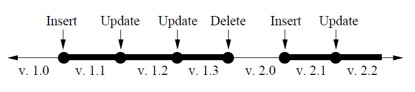
\includegraphics[width=0.8\textwidth]{fig/pnuts-1}
\caption{PNUTS Consistency Model}
\label{fig:pnuts-1}
\end{figure}

\section{Performance}
Bigtable has set up a Bigtable cluster with $N$ tablet servers to measure the performance and scalability of Bigtable as $N$ is varied. $N$ client machines generated the Bigtable load used for these tests. The result is show as Figure \ref{fig:bigtable}, from which implies slowest random read but fast scan since the tablet server can return a large number of values in response to a single client RPC.

\begin{figure}[htbp]
\centering
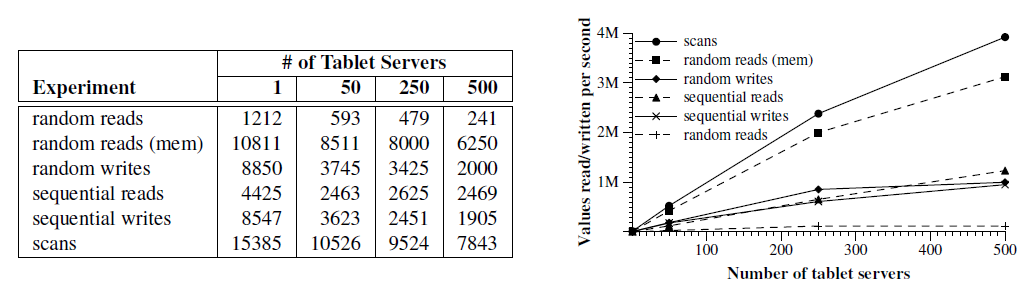
\includegraphics[width=\textwidth]{fig/bigtable}
\caption{Number of 1000-byte values read/written per second. The table shows the rate per tablet server; the graph shows the aggregate rate.}
\label{fig:bigtable}
\end{figure}

Cassandra system tests two kinds of search features: (a) term search (b) interactions.\citep{LakshamAvinash2010} In order to make the searches fast Cassandra provides certain hooks for intelligent caching of data, thus searches (read performance) are dealt within average of 15.69ms and 18.27ms for interactions and term search respectively.\footnote{The system currently stores about 50+TB of data on a 150 node cluster.} However, it doesn't provide any other results.

\citep{Silberstein2008} runs a series of experiments to evaluate the performance of PNUTS. Its performance metric mainly focus on the average request latency. They compared the performance of the hash and ordered tables and get useful lessons about how to improve system. From these results we can see that the performance of ordered tables is better than by hashing.

MongoDB also have done lots of testings. It compares with Postgres and runs much faster when doing simple inserts, since MongoDB does not use transactions or ensures durable writes. A second experiment turns out that MongoDB is really not good at tags search over a lot of data objects.\footnote{Using sharding may improve its performance.} Finally, MongoDB also loses in geospatial queries. Thus, MongoDB is helpful when you need schema-free, or just simple CRUD operations databases.

\section{Chanllenges and Future Works}
Though Dynamo, Cassandra, MongoDB claims to provide scalability, high performance, and wide applicability, there are serveral drawbacks or challenges they currently face.

These systems each optimized for a different point in the design space. Google's Bigtable provides record oriented access to very large tables, but to our knowledge there have been no publications describing support for geographic replication, secondary indexes, materialized views, the ability to create multiple tables, and hash-organized tables. Amazon's Dynamo is a highly-available system that provides geographic replication via a gossip mechanism, but its eventual consistency model does not adequately support many applications, and it does not support ordered tables. Other large scale distributed storage systems include Amazon's S3 and SimpleDB services, and Microsoft’s CloudDB initiative, but there is little information publicly available about the architecture of these systems.

Both PNUTS and Dynamo are distributed data storage systems and are used as scalable back-ends for the various online applications and services of Yahoo and Amazon respectively. The study reveals that both of these systems have some common features and design considerations and are yet distinct with regards to their architectures and implementations.

As for MongoDB, transactions are not directly supported. Other limitations includes that MongoDB does not support full single server durability which means you need multiple replications to avoid data losses if one server suffers a power loss or crash. Another drawback is the fact that it uses much more storage space for the same data then for example PostgreSQL. Because, as opposed to relational databases, every document can have different keys the whole document has to be stored, not only the values. That's why it is recommended to use short key names.

\paragraph*{Indexes and Materialized Views} 
In order to support efficient query processing, it is often critical to provide secondary indexes and materialized views. An index/view maintainer will listen to the stream of updates from message broker, and generate corresponding updates. For example, if a user moves from Wisconsin to California, and we have an index on location, the maintainer will delete the Wisconsin index entry for the user and insert a California index entry for the user. Further research is needed to examine the semantic implications of answering queries using possibly stale indexes and views.

\paragraph*{Bundled Updates} 
Several customers have expressed a need for an extension of the consistency guarantees we provide. The extension, called bundled updates, provides atomic, no isolated updates to multiple records. That is, all updates in the bundle are guaranteed to eventually complete, but other transactions may see intermediate states resulting from a subset of the updates. For example, if Alice and Bob accept a bi-directed social network connection, we need to update both Alice’s and Bob’s records to point to the other user. Both updates need to complete (and the application writer would prefer not to check and retry to ensure this, as in the current system) but it is not critical to provide serializability; it is ok if Alice is temporarily a friend to Bob but not vice-versa. The challenges in implementing bundled updates are to ensure the timeline consistency guarantees described in Section 2.2 when the updates in the bundle are asynchronously and independently applied, and to provide a convenient mechanism for the client to determine when all updates in the bundle have completed.

\paragraph*{Batch-Query Processing}
Although PNUTS is optimized for web OLTP workloads, we believe that it can also serve as a data store for batch and bulk processing, such as that provided by MapReduce or Pig. This requires further investigation of how a scan-oriented bulk workload interacts with a seek-oriented serving workload. It may be necessary to separate PNUTS replicas into ``batch'' and ``serving,'' and optimize them separately for the different workloads. Also, parallel batch systems optimize their execution based on the current location of data, and therefore we may need to provide hooks for accessing tablets directly, bypassing routers.

\section{Conclusion}
The existence of NoSQL has a great deal with Brewer's (CAP) Theorem.\citep{Browne2009} What he said was there are three core systemic requirements that exist in a special relationship when it comes to designing and deploying applications in a distributed environment, and they are \textit{Consistency}, \textit{Availability} and \textit{Partition Tolerance}. The theorem tells us that you can only guarantee two out of three, and that is real and evidenced by the most successful websites as we summarized in sections \ref{majorstream}.

In systems we have covered, of which most favor AP sacrificing C. As cloud computing inevitably involve distributed framework, P is almost a must. Availability is also a necessity when comes to web applications, while consistency is not needed in many cases. However, it does not mean consistency is not important. NoSQL databases still provide ``eventually consistent'' instead as Dynamo and Cassandra does. 

The major goals of NoSQL databases is almost the same: to provide scalable and robust solutions for load balancing, membership and failure detection, failure recovery, replica synchronization, overload handling, state transfer, concurrency and job scheduling, request routing, system monitoring and alarming, and configuration management. On the other hand, different applications vary in requirements of services. Hence, when choosing between SQL and NoSQL, tt really depends on the needs of your application. For web applications that have light querying, key/value stores are very useful. For enterprise databases where reporting is typically very heavy, relational databases fit better. 

\bibliography{refs}

\end{document}